%!TEX root = ../../../../exa-ma-d7.1.tex

\section{Demonstrator: Elliptic linear PDE: CG}

We present here the demonstrator to numerically solve elliptic linear PDE using continuous Galerkin approach.
Precisely, we solve here the heat transfer equation.

\Cref{tab:app-feelpp-discr-1} describes the specifications of the application.

\begin{table}[ht]
    \centering
    \begin{tblr}{
        colspec = {l X[10cm]},
        row{odd} = {numpexlightergray},
        hlines = {0.1pt, numpexgray},
        vlines = {numpexgray},
        row{1} = {numpexgray, fg=white, font=\bfseries},
    }
        Field & Details \\
        id & \texttt{app-feelpp-discr-1} \\
        name & Discretization \\
        Partners & Unistra \\
        PC & PC1 - ExaMA, PC2 - ExaSoft \\
        Responsible (Permanent) & V. Chabannes; C. Prud'homme \\
        WP7 Engineer & Thomas Saigre (UNISTRA) \\
        work\_package & WP1, WP3 \\
        application\_type & extended-mini-app \\
        purpose &  Solve a PDE (heat, solid mech) with different discretization methods from low to high order \\
        Method-Algorithm WP1 & unstructured mesh, finite element, dG/hdG, cG, spectral element \\
        Method-Algorithm WP2 & \\
        Method-Algorithm WP3 & domain decomposition methods, Krylov solver, preconditioning \\
        Method-Algorithm WP4 & \\
        Method-Algorithm WP5 & \\
        Method-Algorithm WP6 & \\
        WP7 & \\
        outputs & Gmsh, JSON config	JSON small-data, JSON reports, in-house, Markdown or Asciidoc \\
        metrics & \texttt{benchmark-verification}, \texttt{strong-scalability}, \texttt{weak-scalability}, \texttt{io-scaling} \\
        status & benchmark-ready \\
        Benchmark scope & full-system, method-verification, solver-scaling \\
        Framework & Feel++, PETSc \\
        parallel\_framework & MPI, Kokkos \\
        spec\_due & 6/15/2025 \\
        proto\_due & 7/1/2025 \\
        repo\_url & \url{https://github.com/numpex/apps-feelpp}\\
    \end{tblr}
    \caption{Description of the demonstrator \texttt{app-feelpp-discr-1}.}
    \label{tab:app-feelpp-discr-1}
\end{table}



\subsection{Description of the benchmark}


The benchmark known as \emph{thermal bridges} is an example of an application that enables us to validate numerical simulation tools using \Feelpp.
We have developed tests based on the ISO 10211:2017 standard \cite{noauthor_iso_2017}, which provides methodologies for evaluating thermal bridges in building construction.

Thermal bridges are areas within a building envelope where heat flow is different compared to adjacent areas, often resulting in increased heat loss or unwanted condensation.
The standard is intended to ensure that thermal bridges' simulation are accurately computed.
It provides reference values and tolerance on heat temperature and heat flux at several locations of the geometry.

At the mathematical level, this application requires finding the numerical
solution of an elliptic linear PDE, namely the heat equation.
We employ a finite element method based on continuous Lagrange Finite Element of order 1,2 and 3 (denoted by $\P_1$, $\P_2$, $\P_3$),
and we analyze the execution time of the main components of the simulation.

\Cref{fig:wp1:feelpp:thermal_bridges:geometry} represents the geometry
of this benchmark and the domain decomposition by material.% the 3D temperature field solution, and an example of mesh partitioning.

\begin{figure}[!ht]
  \centering
  \begin{subfigure}[c]{0.49\textwidth}
    \centering
    \begin{tikzpicture}
        \draw (0, 0) node {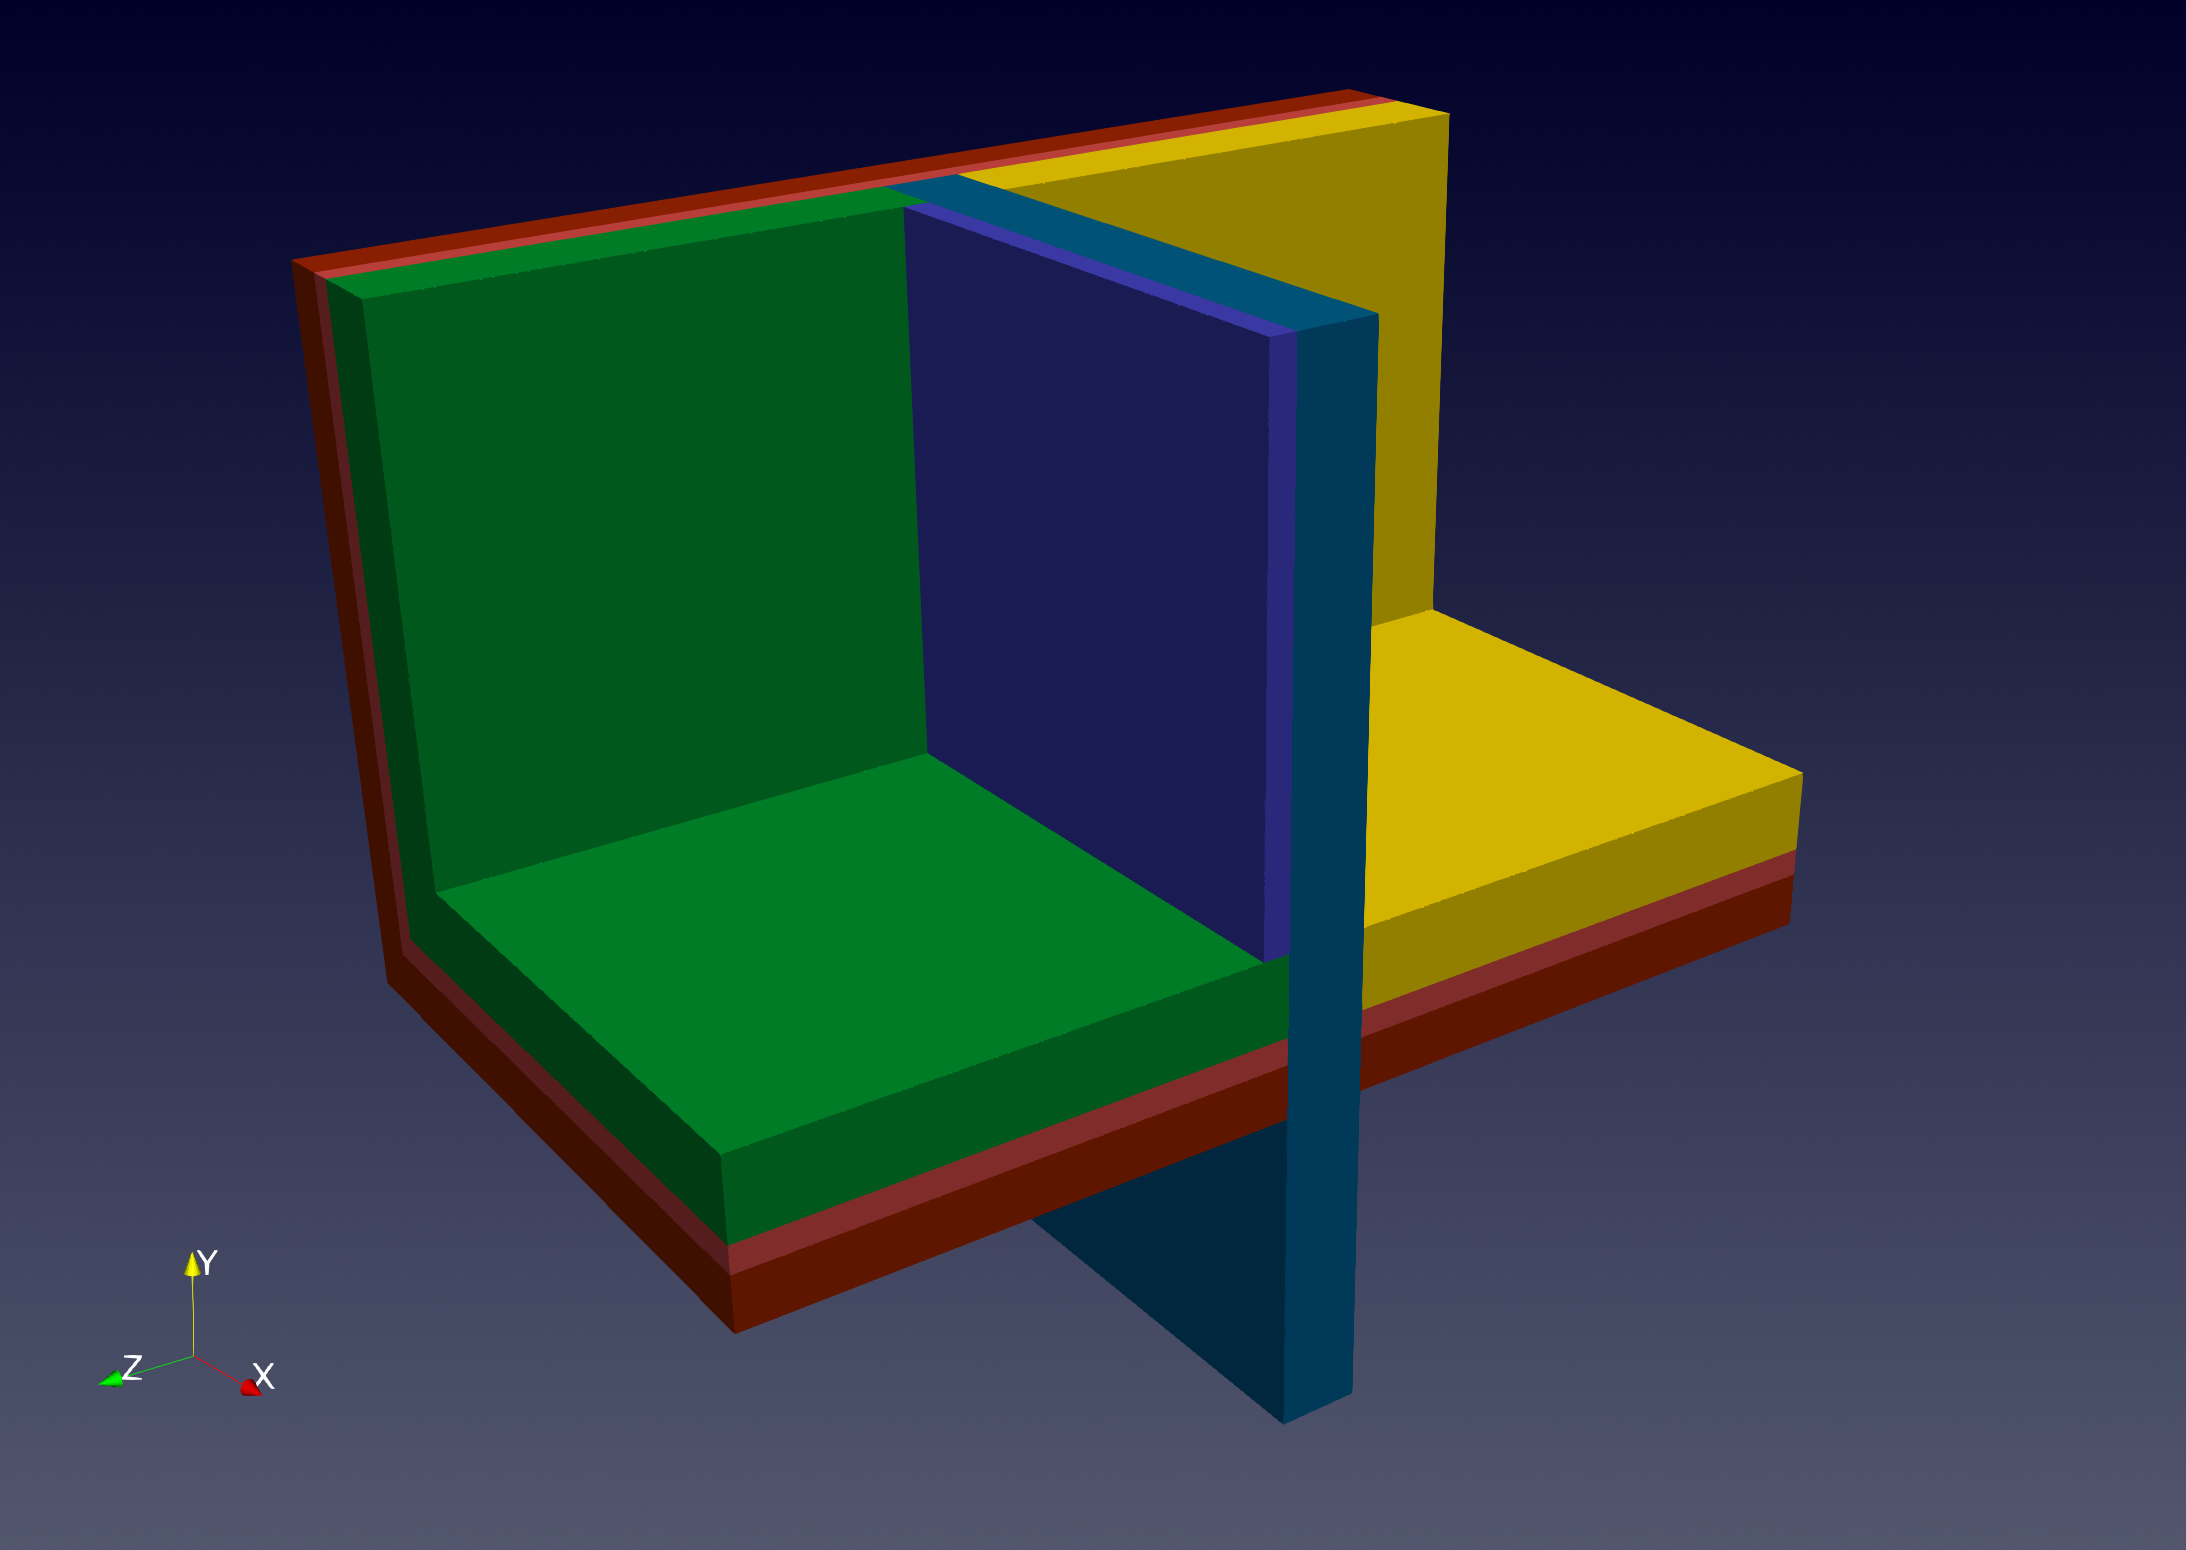
\includegraphics[width=\textwidth]{graphics/feelpp/feelpp-benchmark-thermalbridges-geom.png}};
        \begin{scope}[shift={(2.8, -2.8)}, scale=1.5]
            \draw[red!90!black, ->] (0, 0) -- (0.19, -0.22) node[anchor=west] {$x$};
            \draw[green!70!black, ->] (0, 0) -- (0, 0.4) node[anchor=west] {$y$};
            \draw[blue!80!black, ->] (0, 0) -- (-0.43, -0.07) node[anchor=south] {$z$};
        \end{scope}
    \end{tikzpicture}

  \end{subfigure}
  \hfill
  \begin{subfigure}[c]{0.49\textwidth}
    \centering
        \begin{tikzpicture}
        \draw (0, 0) node {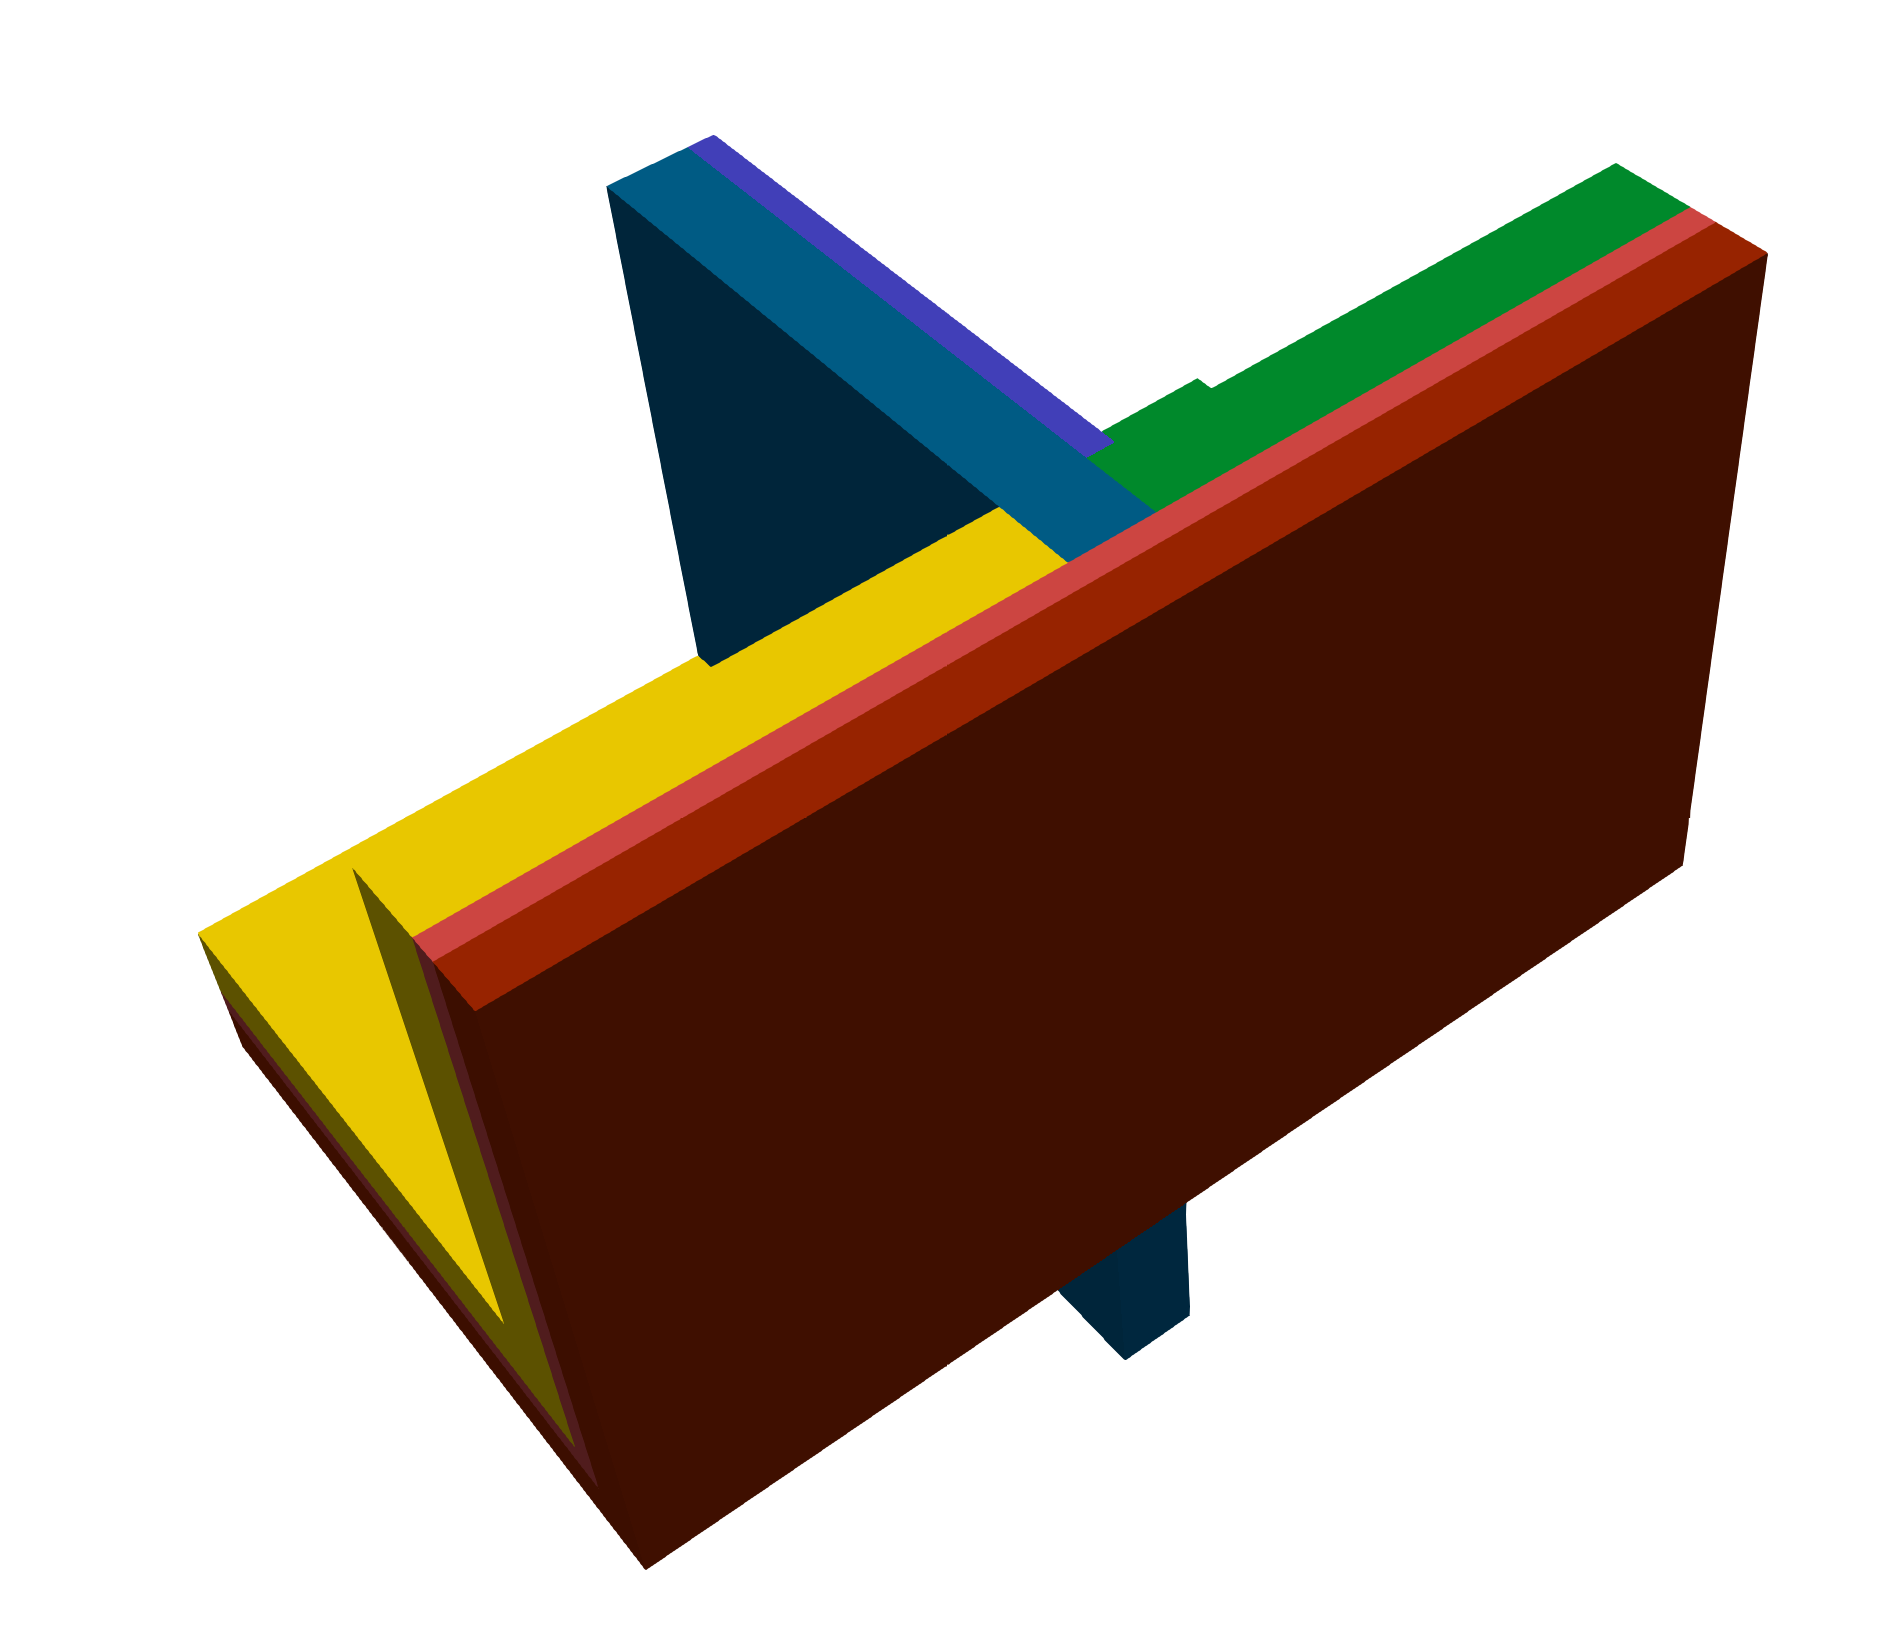
\includegraphics[width=\textwidth]{graphics/feelpp/feelpp-benchmark-thermalbridges-geom2.png}};
        \begin{scope}[shift={(2.8, -2.8)}, scale=1.5]
            \draw[red!90!black, ->] (0, 0) -- (-0.24, 0.22) node[anchor=east] {$x$};
            \draw[green!70!black, ->] (0, 0) -- (-0.04, 0.34) node[anchor=west] {$y$};
            \draw[blue!80!black, ->] (0, 0) -- (0.34, 0.2) node[anchor=north] {$z$};
        \end{scope}
    \end{tikzpicture}
  \end{subfigure}
  \caption{Thermal bridges benchmarks - geometry and materials.}
  \label{fig:wp1:feelpp:thermal_bridges:geometry}
\end{figure}





\subsection{Benchmarking tools used}


The performance tools integrated into the \Feelpp-toolboxes framework were used to measure the execution time.

The metrics measured are the execution time of the main components of the simulation.
We enumerate these parts in the following:
\begin{enumerate}
\item \textbf{Init:} load mesh from filesystem and initialize heat toolbox (finite element context and algebraic data structure).
\item \textbf{Assembly:} calculate and assemble the matrix and right-hand side values obtained using the finite element method.
\item \textbf{Solve:} the linear system by using a preconditioned GMRES.
\item \textbf{PostProcess:} compute validation measures (temperature at points and heat flux) and export on the filesystem a visualization format (EnsighGold) of the solution.
\end{enumerate}




\subsection{Input/Output Dataset Description}


\subsubsection{Input Data:}
  \begin{itemize}
  \item Meshes: We have generated three levels of mesh called \texttt{M1}, \texttt{M2}
    and \texttt{M3}. These meshes are stored in GMSH format. The statistics can be found in \Cref{tab:wp1:feelpp:thermal_bridges:discr_stat}. We have also prepared for
    each mesh level a collection of partitioned mesh.
    The format used is an in-house mesh format of \Feelpp based on
    JSON+HDF5 file type.
    The GMSH meshes and the partitioned meshes can be found on our Girder
    database management, in the \Feelpp collections.
  \item Setup: Use standard setup of \Feelpp toolboxes. It corresponds to a cfg
    file and JSON file. These config files are present in the GitHub of \Feelpp.
  \item Sif image: feelpp:v0.111.0-preview.10-noble-sif  (stored in the GitHub registry of \Feelpp)
  \end{itemize}

\subsubsection{Output Data:}

The output includes the computed values of validation measure in CSV files format, export visualization files (mesh, partitioning, temperature), and the time taken to perform each simulation step.
Metric:
\begin{itemize}
    \item \texttt{benchmark-verification},
    \item \texttt{strong-scalability},
    \item \texttt{weak-scalability},
    \item \texttt{io-scaling}: time taken by the application to read meshes, and to write the solution on disk (especially reading).
\end{itemize}


\SetTblrInner{rowsep=0pt}
\begin{table}[!ht]
    \centering
    \begin{tblr}{
        colspec={c*{7}{Q[c, cmd=\pgfmathprintnumber]}},
        vlines={numpexgray},
        hlines={numpexgray},
        row{1,2}={bg=numpexgray, fg=white, font=\bfseries, halign=c, cmd=\normalfont},
        rowhead=2, % This option excludes the first two rows from the column command
    }
    \SetCell[c=5]{c}{Mesh properties} & & & & & \SetCell[c=3]{c}{Number of degrees of freedom} & &\\
        Tag & \# points & \# edge & \# faces & \# elements & $\Pm_1$ & $\Pm_2$ & $\Pm_3$ \\
        \texttt{M1} & 193654 & 1299920 & 2164759 & 1058492 & 193654 & 1493574 & 4958253\\
        \texttt{M2} & 1401135 & 9778744 & 16566803 & 8189193 & 1401135 & 11179879 & 37525426\\
        \texttt{M3} & 10572256 & 75307308 & 128722252 & 63987199 & 10572256 & 85879564 & 289909124\\
    \end{tblr}

  \caption{Thermal bridges benchmarks - Statistics on meshes and number of degrees of freedom with respect to finite element approximation}
  \label{tab:wp1:feelpp:thermal_bridges:discr_stat}
\end{table}


\subsection{Results summary}


\subsubsection{Numerical solution}

\emph{Insert numerical solution obtained from the toolbox, and the partitioning of the mesh}



\subsubsection{Mesh converging}

\emph{Insert results of mesh converging, with comparison with the reference values of the benchmark \texttt{benchmark-verification}}


\subsection{Times of execution}

\emph{Insert figure with time of execution of the main components described above, for the three meshes (\texttt{strong-scalability}, \texttt{weak-scalability})}


\subsubsection{Scalability on IO}





